%----------------------------------------------------------------------------------------
%	PACKAGES AND OTHER DOCUMENT CONFIGURATIONS
%----------------------------------------------------------------------------------------

\documentclass[
12pt, % The default document font size, options: 10pt, 11pt, 12pt
%oneside, % Two side (alternating margins) for binding by default, uncomment to switch to one side
english, % ngerman for German
onehalfspacing, % Single line spacing, alternatives: singlespacing, onehalfspacing or doublespacing
%draft, % Uncomment to enable draft mode (no pictures, no links, overfull hboxes indicated)
nolistspacing, % If the document is onehalfspacing or doublespacing, uncomment this to set spacing in lists to single
liststotoc, % Uncomment to add the list of figures/tables/etc to the table of contents
%toctotoc, % Uncomment to add the main table of contents to the table of contents
parskip, % Uncomment to add space between paragraphs
%nohyperref, % Uncomment to not load the hyperref package
headsepline, % Uncomment to get a line under the header
%chapterinoneline, % Uncomment to place the chapter title next to the number on one line
consistentlayout, % Uncomment to change the layout of the declaration, abstract and acknowledgements pages to match the default layout
]{MastersDoctoralThesis} % The class file specifying the document structure


\usepackage[utf8]{inputenc} % Required for inputting international characters
\usepackage[T1]{fontenc}

\usepackage{mathpazo} % Use the Palatino font by default
\usepackage{color}
\usepackage{subfigure}
\usepackage{array}
\usepackage{listings}
\usepackage{amssymb}
\usepackage{ifthen}
\usepackage{float}
\usepackage{lscape}
\newcolumntype{C}[1]{>{\centering\let\newline\\\arraybackslash\hspace{0pt}}m{#1}}
\newcolumntype{L}[1]{>{\centering\let\newline\\\arraybackslash\hspace{0pt}}p{#1}}
\usepackage{hyperref}
\lstset{numbers=left, basicstyle=\footnotesize, frame=single, breaklines=true, breakatwhitespace=true}

\usepackage[backend=bibtex]{biblatex} % Use the bibtex backend with the authoryear citation style (which resembles APA)


\addbibresource{example.bib}

\usepackage[autostyle=true]{csquotes} % Required to generate language-dependent quotes in the bibliography

\newcommand{\projectName}{\textbf{ProjectName} }

%----------------------------------------------------------------------------------------
%	MARGIN SETTINGS
%----------------------------------------------------------------------------------------

\geometry{
	paper=a4paper, % Change to letterpaper for US letter
	inner=2.5cm, % Inner margin
	outer=3cm, % Outer margin
	bindingoffset=.5cm, % Binding offset
	top=1.5cm, % Top margin
	bottom=1.5cm, % Bottom margin
	%showframe, % Uncomment to show how the type block is set on the page
}

%----------------------------------------------------------------------------------------
%	THESIS INFORMATION
%----------------------------------------------------------------------------------------

\thesistitle{Comparison and Analysis Between Automatic Exploration Tools for Android Applications} % Your thesis title, this is used in the title and abstract, print it elsewhere with \ttitle
\supervisor{Mario \textsc{Linares-Vásquez}} % Your supervisor's name, this is used in the title page, print it elsewhere with \supname
\examiner{} % Your examiner's name, this is not currently used anywhere in the template, print it elsewhere with \examname
\degree{Bachelor in Software and Computer Engineering} % Your degree name, this is used in the title page and abstract, print it elsewhere with \degreename
\author{Michael \textsc{Osorio-Riaño}} % Your name, this is used in the title page and abstract, print it elsewhere with \authorname
\addresses{} % Your address, this is not currently used anywhere in the template, print it elsewhere with \addressname

\subject{Biological Sciences} % Your subject area, this is not currently used anywhere in the template, print it elsewhere with \subjectname
\keywords{} % Keywords for your thesis, this is not currently used anywhere in the template, print it elsewhere with \keywordnames
\university{\href{http://uniandes.edu.co}{University of Los Andes}} % Your university's name and URL, this is used in the title page and abstract, print it elsewhere with \univname
\department{\href{http://sistemas.uniandes.edu.co}{Systems and Computing Engineering Department}} % Your department's name and URL, this is used in the title page and abstract, print it elsewhere with \deptname
\group{\href{https://ticsw.uniandes.edu.co/}{TICSw research group}} % Your research group's name and URL, this is used in the title page, print it elsewhere with \groupname
\faculty{Faculty of Engineering} % Your faculty's name and URL, this is used in the title page and abstract, print it elsewhere with \facname

\AtBeginDocument{
\hypersetup{pdftitle=\ttitle} % Set the PDF's title to your title
\hypersetup{pdfauthor=\authorname} % Set the PDF's author to your name
\hypersetup{pdfkeywords=\keywordnames} % Set the PDF's keywords to your keywords
}


\definecolor{orange}{rgb}{1,0.5,0}

\makeatletter

% this  is a easy way to add and highlight new text  ...
% just comment in/out the \tnew macro ..

\newcommand{\tnew}[1]{{\bf { #1 }} }
%\newcommand{\tnew}[1]{{ { #1 }} }

% math and theorem definition

\newcommand{\ndef}{\stackrel{\rm def}{=}}

% this is used for draft only

%\renewcommand{\baselinestretch}{2}

% just to number pages in the draft

\pagenumbering{arabic}

% nothing i.e., no-numbering final and camera ready

%\pagestyle{empty}


\newboolean{showcomments}


\setboolean{showcomments}{true}

\ifthenelse{\boolean{showcomments}}
  {\newcommand{\nb}[2]{
    \fbox{\bfseries\sffamily\scriptsize#1}
    {\sf\small$\blacktriangleright$\textit{#2}$\blacktriangleleft$}
   }
   \newcommand{\cvsversion}{\emph{\scriptsize$-$Id: macro.tex,v 1.9 2005/12/09 22:38:33 giulio Exp $}}
  }
  {\newcommand{\nb}[2]{}
   \newcommand{\cvsversion}{}
  }



\newcommand\CAMILOO[1]{\textcolor{red}{\nb{CAMILO}{#1}}}
\newcommand\CAMILO[1]{\textcolor{orange}{\nb{CAMILO}{#1}}}

\newcommand\MARIO[1]{\textcolor{red}{\nb{MARIO}{#1}}}

\newcommand{\cmark}{\ding{51} }%
\newcommand{\xmark}{\ding{55}}%
\newcommand\fix[1]{\textbf{FIX THIS}{#1}}
\newcommand{\here}{\textcolor{red}{\textbf{***}{CONTINUE HERE}}}
\newcommand{\ie}{\textit{i.e.,}\xspace}
\newcommand{\eg}{\textit{e.g.,}\xspace}
\newcommand{\etc}{\textit{etc.}\xspace}
\newcommand{\etal}{\textit{et al.}\xspace}
\newcommand{\libra}{{\sc Libra}\xspace}
\newcommand{\secref}[1]{Section~\ref{#1}\xspace}
\newcommand{\chapref}[1]{Chapter~\ref{#1}\xspace}
\newcommand{\appref}[1]{Appendix~\ref{#1}\xspace}
\newcommand{\figref}[1]{Fig.~\ref{#1}\xspace}
\newcommand{\listref}[1]{Listing~\ref{#1}\xspace}
\newcommand{\tabref}[1]{Table~\ref{#1}\xspace}
\newcommand{\sotag}[1]{<#1>\xspace}
\newcommand{\todoref}{\textcolor{red}{[REF]}}
\newcommand{\tool}{\texttt{MutAPK} \xspace}




\begin{document}

\frontmatter % Use roman page numbering style (i, ii, iii, iv...) for the pre-content pages

\pagestyle{plain} % Default to the plain heading style until the thesis style is called for the body content

%----------------------------------------------------------------------------------------
%	TITLE PAGE
%----------------------------------------------------------------------------------------

\begin{titlepage}
\begin{center}


% {\scshape\LARGE \univname\par}\vspace{1.5cm} % University name
\begin{figure}[h]
\centering

\includegraphics[width=0.4\textwidth]{../Figures/logoUniandes}
\end{figure}
%\vspace*{.07\textheight}
%\textsc{\Large Master Thesis}\\
\vspace{0.3cm} % Thesis type

\HRule \\[0.4cm] % Horizontal line
{\huge  \ttitle\par}\vspace{0.4cm} % Thesis title
\HRule \\[1cm] % Horizontal line
 
\begin{minipage}[t]{0.4\textwidth}
\begin{flushleft} \large
\emph{Author:}\\
\href{https://michaelosorio2017.github.io/}{\authorname} % Author name - remove the \href bracket to remove the link
\end{flushleft}
\end{minipage}
\begin{minipage}[t]{0.3\textwidth}
\begin{flushright} \large
\emph{Advisor:} \\
\href{https://profesores.virtual.uniandes.edu.co/mlinaresv/en/inicio-en/}{\supname} % Supervisor name - remove the \href bracket to remove the link  
\end{flushright}
\end{minipage}\\[1.5cm]
 
\vfill

\large \textit{A thesis submitted in fulfillment of the requirements\\ for the degree of \degreename}\\%[0.1cm] % University requirement text
\textit{in}\\%[0.3cm]
%\groupname
\begin{figure}[h]
\centering

\includegraphics[width=0.5\textwidth]{../Figures/tsdlLargo}
\end{figure}
\deptname\\[0.5cm] % Research group name and department name
 
\vfill

{\large \today}\\
%[4cm] % Date
%\includegraphics{F} % University/department logo - uncomment to place it
 
\vfill
\end{center}
\end{titlepage}


%----------------------------------------------------------------------------------------
%	ABSTRACT PAGE
%----------------------------------------------------------------------------------------

\begin{abstract}
\addchaptertocentry{\abstractname} % Add the abstract to the table of contents
The number of different tools to explore Android applications has been increasing. Every tool has a different exploration strategy and clam to offer different benefits than others. The huge amount of tools and the lack of impartial information about them makes that developers and researchers has no the basis and data to face a decision-making situation or data to compare their own new tool. 
Others studies have made different comparisons between exploration tools in the past, but most of those tools are not longer being use by the industry or by the academy, that is why there is a need of studies providing clear and unbiased information about the newest tools that allows the developers and researchers to acquire a better perspective of the modern exploration tools. 
That is the reason why in this study, four of the most used tools for automatic exploration of Android applications are analysed and compared according their method coverage reached and their number of errors found. Besides, a reproducible work flow is proposed for future studies of the same type as well as two tools for allowing faster and easier comparison are described.
\end{abstract}

%----------------------------------------------------------------------------------------
%	ACKNOWLEDGEMENTS
%----------------------------------------------------------------------------------------

\begin{acknowledgements}
\addchaptertocentry{\acknowledgementname} % Add the acknowledgements to the table of contents

First, I want to express my deepest thanks to Professor Mario Linares-Vásquez for helping me with the development of this final work, giving me the necessary feedback for getting this project to this final version. Giving me new ideas and ways to solve the presented problems while executing this research.

Second, I would like to give my thanks to all the members of The Software Design Lab, for sharing with me their experiences and knowledge which were very important for developing this thesis. Especially to Camilo Escobar for his great help giving the main concept of InstruAPK, for helping with its implementation, besides giving me feedback about the figures in this text as well as solving some extra questions and doubts that I had during the process of developing this thesis.

Third, I want to say thanks to my mother and sister for keeping me motivated within all my major, till the last moment of it. For their unconditional support and for being there in the moments I needed them the most. 

At last, but not least important, I want to say thanks to all my friends for sharing their knowledge with me, and contributing with that to the final product of this thesis. 

Without the help of the mentioned people, this work would not be possible.

I wish to clarify that the order in the mention does not reflect the level of thankfully I feel for the people mentioned in this statement. All of them supported this work in different ways, and under their capabilities, helping me in one way or another to reach this results. For that reason, all of them deserve the same feelings from my. One more time, thanks to all of them.
\end{acknowledgements}

%----------------------------------------------------------------------------------------
%	LIST OF CONTENTS/FIGURES/TABLES PAGES
%----------------------------------------------------------------------------------------

\tableofcontents % Prints the main table of contents

\listoffigures % Prints the list of figures

\listoftables % Prints the list of tables


%----------------------------------------------------------------------------------------
%	SYMBOLS

%----------------------------------------------------------------------------------------
%	THESIS CONTENT - CHAPTERS
%----------------------------------------------------------------------------------------

\mainmatter % Begin numeric (1,2,3...) page numbering

\pagestyle{thesis} % Return the page headers back to the "thesis" style

% Include the chapters of the thesis as separate files from the Chapters folder
% Uncomment the lines as you write the chapters

% Chapter Template

\chapter{Introduction} % Main chapter title

\label{Chapter1} % Change X to a consecutive number; for referencing this chapter elsewhere, use \ref{ChapterX}

\MARIO{CITE Statista}
Mobile applications market is a continuous growing market. According to Statista, the number of available applications, by the 2020, in the two main markets together is 4407000. The large amount of applications means that there is a vast number of users willing to download them, but also it means that they can change an application, or even the platform, whenever they desire to, or when something does not fulfil their needs or expectations. Therefore, every day more and more complex applications are released in the market as well as the users becomes more demanding. As a result, every new application or new functionality should have a good quality, they should work as expected in all different scenarios the distinct users will put them in, they have to be developed very fast and also, they have to be cheap in order to be sustainable for the company who develops them. 

The large amount of publicly available, their complexity, and also the more demanding users make this market a very competitive one.

In order to reach users quality expectations, improve release times  and the sustainability needed for the companies, many approaches have been promoted, among them, automated testing. Automated testing has been of high interest for researchers and companies because it lowers the costs of production and it allows better quality products. One of the branches of automated testing is automatic exploration tools; these tools aim to explore  applications as deep as possible and find as many errors as possible. There is a plethora of exploration tools. Every year there are more of them, each one using different exploration strategies. Some of them use random inputs, others use image analysis, others use a mixture of these two, and new researches are starting using AI. It is easy to think that the more deep the exploration the more errors will be found, however, as will be shown in this text, that is not always the case. The number of errors detected can vary due to the exploration strategy because of the nature of the errors  and the apps. Furthermore, most of the exploration tools are developed for Android applications.

Examples of the automatic exploration tools are Monkey \footcite{https://developer.android.com/studio/test/monkey}. This tool uses a pseudo-random generation events strategy, leading to different exploration results unless the same seed is given for the generation of the random events. This tool is the default one provided by Google. Another well known tool is Firebase Test Lab \footcite{https://firebase.google.com/}; this tool can be used online. Accordingly to its documentation, it analyzes the UI of the applications and explores the apps by simulating users events. They claim to always explore the tool in the same order. Another exploration tool is RIP \MARIO{CITE. USE THE PAPER CAMILO SAID}, an active project from  The Software Design Lab at \emph{Universidad de los Andes}; RIP explores applications using a model-based GUI testing technique. It can lead to different exploration results due to its current implementation as well as to the comparison criteria. 

For developers, it  is important to know the difference between these tools. They need to know the tools that will work the best in the new incoming project to make a good decision. Besides, the project budget, and application complexity among others things can also affect the decision. The information available to make the decision is often based in what the tools claim to do. This information is not completely reliable.

Additionally, for researchers, it is also important to know what is the advantages of all the different exploration strategies, as well as their disadvantages. They need to compare them to know what is the next step to make the field go further.

%----------------------------------------------------------------------------------------
%	SECTION 1
%----------------------------------------------------------------------------------------

\section{Problem Statement}

Accordingly to the previous section, the number of automatic exploration tools is increasing annually. Thus, with no objective information about them, developers  will need to explore new tools and compare them to find the best one. It can turns easily in spending valuable time and at the end in making the wrong decision, resulting in final products with poor quality. In short, the decision of the right automatic exploration tool should be easy and rely in objective data, such as coverage reached, and number of errors found.

\section{Thesis  Goals}\label{sec:thesisGoals}

The main objective of this thesis, is to provide quantitative and qualitative information of the most widely used automatic exploration tools for Android mobile applications, to facilitate developers in the selection of the right tool that suits their needs. Under those circumstances, the following specific objectives were proposed:
		\begin{enumerate}
			\item Compare exploration tools  based on their method  coverage capabilities
			\item Compare exploration tool based on the number of unique error traces discovered while exploring an application.
		\end{enumerate}

\section{Thesis contribution} \label{sec:thesisContribution}

The main contribution of this thesis is to provide developers with enough objective information, to decide which automatic exploration tool suits the most their projects' needs, making this process easy and less time consuming.

Alongside, this study shows that higher coverage does not guaranties higher number of found errors, which, as shown later in this work, is the case of Firebase Test Lab. This tool had the highest method coverage both in average and accumulated, but it is not the best one when regarding to errors found. 

All this information provides better points of view to developers and researchers, giving fixed and objective comparison points that they can use in a decision-making situation, resulting in better projects. 

Furthermore, even when the study does not have the objective of create a reproducible work flow, it was created. New researches can use it as a base for new comparison studies, as well as extend it, and enhance it to create a new standardization of the validation of new exploration tools for Android applications. Plus, two tools for helping the validation of new exploration tools were designed InstruAPK (section \ref{sec:instruAPK}) and CoverageAnalyzer (section \ref{sec:ca}). Such tools also can be improved, adding more features and gaining more and preciser information from the explorations.
	
\section{Document Structure}

This document has the following structure: In Chapter \ref{Chapter2} related work is described, you will find information about automatic exploration tools for android applications as well as information about researches that have already made comparisons between some tools. Next chapter, Chapter \ref{Chapter3} describe the solution design which includes, the general approach (Section \ref{sec:generalApproach}) to get done the objectives described in section \ref{sec:thesisGoals}, besides a brief explanation of the tools created for this study (Sections \ref{sec:instruAPK} and \ref{sec:ca}). Now, in chapter \ref{Chapter4} you will find the empirical study, here is clarify how the data was obtained, what tools and applications were used, the devices involved in the study and other important data to reproduce the research. Additionally, in the same chapter you will find the results of the study together with their reasoning. On top of that, chapter \ref{Chapter5} describes de conclusions using the data obtained in the previous chapter. Finally, chapter \ref{Chapter6} depicts the future work, discoursing the new researches that could be made when taking this study as a base or as a reference.

% Chapter Template

\chapter{Related work} % Main chapter title
\label{Chapter2} % Change X to a consecutive number; for referencing this chapter elsewhere, use \ref{ChapterX}

%---------------------------------------------------------------------------------------
%	SECTION 1
%----------------------------------------------------------------------------------------

Every exploration tool provides different numbers, and comparisons made during their creation, this in order to show their advantages, but not for sure their weaknesses. This information does not allow developers neither researchers to know what are the best tools as of now or how good a tool matches their projects. 
S.R. Choundhary \textit{et al} \cite{Choudhary} gave informations about the strengths and weaknesses of seven tools in their study \textit{``Automated Test Input Generation for Android: Are We There Yet?``}. They evaluated the tools using four metrics i. ease
of use, ii. ability to work on multiple platforms, iii. code coverage, and iv.
ability to detect faults. 14 Tools and 68 applications were used in total in their study. Running 10 times every application in seven of the 14 tools for a maximum of 60 minutes.

Moreover, different tools have been developed since \cite{Choudhary} study was made.

\section{Crawldroid}\label{sec:crawldroid}

Crawldroid \cite{Cao} uses a model-based GUI testing technique. Its purpose is to avoid local and repetitive exploration, by grouping widgets and then adjust the groups priority depending on previous steps and the results of the widgets already actioned. 

This tool makes part of a study named \textit{``CrawlDroid: Effective Model-based GUI Testing of Android Apps``}where the authors made a comparison between this tool and some others in order to know how good is their tool. Using a tool called ELLA \footnote{https://github.com/saswatanand/ella} for its coverage measurement. ELLA provides information about method and activity coverage.

Crawldroid was not used in this study because it was not possible to make it work. The setup of the tool was not possible. The were tries to contact with the authors but no answer was received from them.

\section{Droidbot}\label{sec:droidbot}
Droidbot \cite{droidbot} is a Lightweight exploration tool that does not need instrumentation in order to work. Droidbot is able to generate UI-guided test inputs using a state transition model that is generated while exploring the application. It is a open source project.

This tool is also a open source project and it makes part of a study, where their authors explains that the tool can calculate different metrics by using the Android official profiling tool. Their approach can follow the trace of the methods that are triggered when a new widget is clicked or when a event is prompt. Besides, if the number of methods is available they will also calculate the coverage reached in the exploration.

\section{Firebase Test Lab}\label{sec:testlab}

Firebase Test Lab \footnote{https://firebase.google.com/}, is a Google product. This tool is different to the others because it does not make part of research and also because it is available in the cloud, the users should create an account on it, create a project, upload the apk and the run the test. This is the unique exploration tool that is run in this way. Different from the other tools mentioned in this chapter, this is the only one that has a paid version. It reports no coverage values, but number of visited activities.

\section{RIP}\label{sec:rip}
RIP \cite{Liñán} is an active project at The University of Los Andes in charge of The Software Design Lab, this tool is designed to take into account multiple variables during the exploration. Variables such as, context of the application while exploring an activity, the GUI elements presented in one activity. The purpose of this extra information is to provide a better quality testing.

This tool is also part of a research named \textit{``Automated Extraction of Augmented Models for Android Apps``}. where their authors claim that all this new information is necessary owing to the complexity of mobile applications. Thus, when more information is recorded and less variables are unknown, bugs reproduction will be easier.

RIP does not contains any coverage metrics by default, its coverage should be calculated by using a different tool. It only provides information about what activities visited, what events triggered to get from one state to another, and some other extra information later discussed.

As can be seen, non of the aforementioned tools were discussed in S.R. Choudhary \textit{et al} \cite{Choudhary} work. Most probably because by the time they made the research, none of them existed. This creates a gap between the available information for developers and researches and the current automatic exploration tools. As a result, this study aims to provide information about some of the newest tools that are being used in the industry and the academy. Giving a better overview of nowadays automatic exploration tools.

% Chapter Template

\chapter{Solution Design} % Main chapter title

\label{Chapter4} % Change X to a consecutive number; for referencing this chapter elsewhere, use \ref{ChapterX}

\section{General Approach} \label{sec:generalApproach}

With the aim of complete the specific objectives and thus the main one, all of them mentioned in Sec.\ref{sec:thesisGoals}, a workflow was designed. This work flow contains five stages.

\begin{enumerate}
	\item The applications were instrumented using \textbf{InstruAPK.}
	\item The exploration was made using Droidbot, Monkey, RIP and Firebase Testlab
	\item The coverage measurement was made using \textbf{CoverageAnalyzer (CA).}
	\item Summarize data. Total number of unique methods called during all ten executions, reporting only the first time they were called.
	\item Understanding data, computing statistics, creating graphs, extract insights and concluding.
\end{enumerate}

Stages 2. and 3. were repeated 10 times for every application that was selected, that leaded to the stage iv. The multiple executions are intending to get average values as well as better comparable results along the different exploration tools.

\begin{figure}[h]
\centering
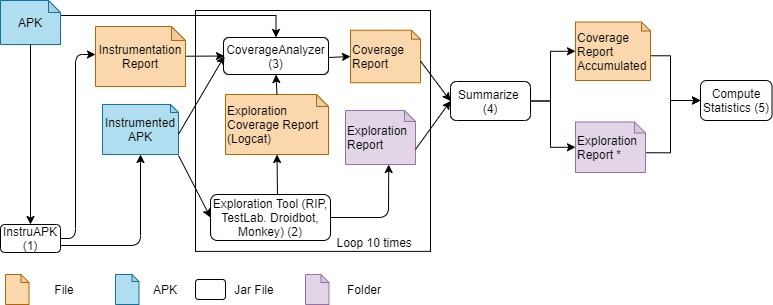
\includegraphics[width=0.8\textwidth]{../Figures/workflow.jpg}
\label{fig:workflow}
\caption{Main Workflow}
\end{figure}


explicar el workflow de cómo se obtuvieron los resultados.

\textbf{APK processing.} 

In order to measure the method coverage reached by an exploration tool in one application, there is the need to know how many methods there are in the application and how many methods were called during the exploration. To achieve that, \textbf{InstruAPK.} and \textbf{CoverageAnalyzer (CA).} were developed.
%TODO citate InstruAPK repository
%TODO citate CA repository

\section{InstruAPK}

Instrumentation tool developed mainly for this study. This tool uses APKTool, a known Java application that allows inverse engineering in Android apps, allowing applications' instrumentation without the need of recompiling their source code. APKTool decodes the apk and the result is the smali representation of the app source code, These smali files are analysed in order to find all the methods to be instrumented and then, the log code is injected at the very beginning of each method. Its important to notice that no external libraries methods are instrumented. InstruAPK only search for methods following the android project structure that uses the application package name to store the application source code.

\begin{figure}[h]
\centering
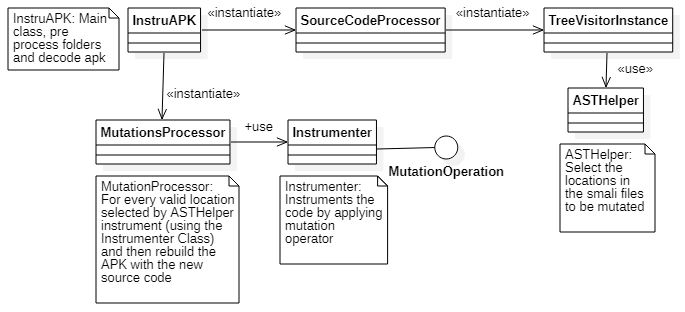
\includegraphics[width=0.8\textwidth]{../Figures/ClassDiagramInstruAPK.jpg}
\label{fig:instruAPK}
\caption{Class Diagram InstruAPK}
\end{figure}

%TODO explain the architecture and the tool in more detail, do not throw the image and just that.
\section{Coverage Analyser (CA)}

Java Application created mainly for this study. This tool extracts all data from the log lines injected by InstruAPK. When an instrumented application is ran, the logcat will contain the log lines with all the data. The logcat is stored in a txt file and that is what CA uses as its input. As CA depends totally on the information provided by InstruAPK, CA can be seen as a complement of it, rather than an separate application.

\begin{figure}[h]
\centering
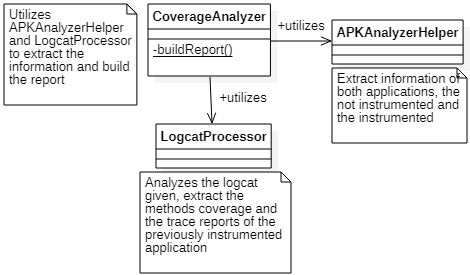
\includegraphics[width=0.8\textwidth]{../Figures/ClassDiagramCA.jpg}
\label{fig:ca}
\caption{Class Diagram Coverage Analyser}
\end{figure}
%TODO explain the architecture and the tool in more detail, do not throw the image and just that.
% Chapter Template

\chapter{Empirical Study} % Main chapter title

\label{Chapter5} % Change X to a consecutive number; for referencing this chapter elsewhere, use \ref{ChapterX}

%----------------------------------------------------------------------------------------
%	SECTION 1
%----------------------------------------------------------------------------------------
\section{Study Design}

Comenzar con los objetivos de la tesis.
Explicar por qué se seleccionaron las herramientas (RIP, TestLab, etc)
Explicar las apps utilizadas en el estudio.
explicar el workflow de cómo se obtuvieron los resultados.
mostrar los resultados y analizarlos.

In order to measure the method coverage reached by an exploration tool in one application, there is the need to know how many methods there are in the application and how many methods were called during the exploration. To achieve that, the application developers could count the number of methods in their project and write log lines at the beginning of every method. After that, they will need to compile, run the exploration tool against their application, measure the number of methods that were called during the exploration and compute statistics.

With that in mind, this study consists of nearly the same stages, i. instrumentation, ii. exploration, iii. coverage analysis, iv. summarize, and v. compute statistics. The stages ii. and iii. were repeated 10 times for every application that was selected, that leaded to the iv. stage.

The different stages were completed as follow:

Stage i: The applications' instrumentation was made by using InstruAPK. It is an instrumentation tool developed mainly for this study. This tool uses APKTool, a known Java application that allows inverse engineering in Android apps, allowing applications' instrumentation without the need of recompiling their source code. APKTool decodes the apk and the result is the smali representation of the app source code, These smali files are analysed in order to find all the methods to be instrumented and then, the log code is injected at the very beginning of each method. Its important to notice that no external libraries methods are instrumented. InstruAPK only search for methods following the android project structure that uses the application package name to store the application source code.

Stage ii: The exploration was made by four different automatic exploration tools. two from the industry and two from the academic side. The first tool was Firebase Test Lab. it was selected for being widely used in industry and for also being a Google product. The second one, Monkey, was selected for being the most basic one and because it is also included in the SDK for developing Android Apps. The third one, Droidbot, was selected from the academic side. Droidbot has been a point of study for many researches. Many others tools have based their functionality on this tool. The last one is RIP, this tool was selected for being of special interest for us. It is our own exploration tool and is is currently an active project inside the Software Design Lab at University of Los Andes. 

Every tool was executed ten times per application, and every execution with a maximum time of 30 minutes. Some tools ended its exploration before the max time. 
The number of executions and the maximum time were arbitrary decisions that were made because of time limitations for the study. Although, during the study was notice that most of the tools ended the exploration or reached their maximum coverage within the first 15 minutes. Which means that the maximum time for exploration was more than enough in almost all cases. 
 
stage iii: The coverage measurement was made by CoverageAnalyzer. It is a Java Application created mainly for this study. This tool analyses the resulting logcat of an Android phone, when executing an application that was instrumented by InstruAPK. It extracts different data such as, number of methods called, number of  methods never called, number of error traces of the application being analysed, most called methods, less called methods, as well as the time stamp of all calls of every method. It is important to notice that the possibility of extracting all those information is because InstruAPK provides it.

stage iv: Due to the multiple executions of every APK per tool, it is important to summarize de data. The final report contains the total number of unique methods called during all ten executions, reporting only the first time they were called.
The exploration reports are analysed and filtered as well.

stage v: This is the final stage of the study that involves, understanding data, computing statistics, creating graphs, extract insights and conclusions. 

Besides that, for this study, a set of 11 applications was used. This set is a subset of a set of open source applications utilised inside The Software Design Lab research group for other studies and tests, including RIP. Every APK in the subset should be successfully instrumented by InstruAPK, it should compile without any problem after instrumentation and it should be launch in an emulator without any issue after instrumentation.

\section{Context of the Study}

In order to present a fair comparison between MutAPK and MDroid+, we have used the same apps MDroid+ used for their experiments. This 54 applications presented in Table \ref{tab:alufs} belong to 16 different categories of the Google Play Store. It is worth noticing that these 54 applications are open source and allows us to study the way code statements are translated from JAVA to SMALI.

In order to collect data that allow us to answer the research question, we compared MutAPK to an existing tool for mutation testing that works at source code level ( MDroid+ \cite{linares2017enabling} ). 
The experiments were executed on a class-server machine. 
Note that in MutAPK, we implemented only 35 of 38 operators listed in Table \ref{tab:cmol} because the other 3 operators lead to non-compilable results. In order to analyze the impact of mutant generation process in MutAPK, we collect: (i) number of mutants generated per mutation operator per application; (ii) number of mutants that compile after mutation; (iii) mutant generation time (\textit{i.e.,} the time required to generate each mutant) and (iv) mutant building times (\textit{i.e.,} the time required to compile each APK file)
\begin{table}[t]
	\centering
	\caption{Applications used for the study}
	\label{tab:alufs}
	\resizebox{0.80\textwidth}{!}{
		\begin{tabular}{c c c c}
			App ID & Package Name & \# Methods Reported by APKAnalyzer & \# Methods Instrumented by InstruAPK\\
			\hline
			1 & appinventor.ai\_nels0n0s0ri0.MiRutina & 61993 & 9351\\
			2 & com.evancharlton.mileage & 4000 & 1162\\
			3 & com.fsck.k9 & 18799 & 7003\\
			4 & com.ichi2.anki & 32370 & 2209\\
			5 & com.workingagenda.devinettes & 19274 & 66 \\
			6 & de.vanitasvitae.enigmandroid & 13083 & 574 \\
			7 & info.guardianproject.ripple & 19429 & 100 \\
			8 & org.connectbot & 20606 & 1145\\
			9 & org.gnucash.android & 75473 & 504\\
			10 & org.libreoffice.impressremote & 14691 & 649\\
			11 & org.lumicall.android & 45784 & 540\\
			\hline
		\end{tabular}
	}
\end{table}

\section{Results: Impact of generating mutants at APK level}

\textbf{\textit{$RQ_{1.1}$}}: To study our results, we present them in two stages, first we show a comparison where only the 33 mutants  in both MDroid+ and MutAPK are taken into account. In Figure \ref{fig:s22agmbp} we show the total amount of generated mutants per app. MutAPK generates around 30 more mutants per app (17\% more than MDroid+). However, if all operators are taken into account, the difference between the amount of mutants get bigger. Figure \ref{fig:agmbp} shows the amount of generated mutants per app. As it can be seen, MutAPK outperforms MDroid+ generating in average 1211 more mutants per app, this corresponds to 7.3 times more mutants. For further analysis of the results at app level, we added the Tables \ref{tab:cal1} and \ref{tab:cal2}, where all info collected is summarized around apps (See Appendix A). Also, we show in Figure \ref{fig:s22agmmobp} that the amount of mutants generated per mutant operator are very similar between MutAPK and MDroid+. It is worth nothing that this figure does not take into account the 63441 mutants generated by one of the operators implemented only in MutAPK. 

\textbf{\textit{$RQ_{1.2}$}}: If we consider again only the 33 shared mutants, in Figure \ref{fig:s22pncmbp} we can see that MutAPK generates around 16\% of non-compilable mutants while MDroid+ generates only 0.5\%. Nevertheless, when using all operators MutAPK generates around 2.36\% of non-compilable mutants while MDroid+ lightly increase its rate to 0.6\%. At the same time, Figure \ref{fig:s22pncmmobp} shows the percentage of non-compilable mutants in terms of the mutant operators, from this we can see that there is also a similar behavior for both. Specifically, MutAPK generates in average 0.1\% non-compilable mutants while MDroid generates 0.05\%.

\textbf{\textit{$RQ_{1.3}$}}: The most important result is the execution time. MutAPK takes only 3\% of the time ( 144,66ms ) required by MDroid+ ( 4,6 seconds) to mutate a copy of the app. Therefore, due to the infraestructure used to run our study, MutAPK takes 9 seconds to generate all mutants for an app (on average), while MDroid takes 19 seconds. 

\textbf{\textit{$RQ_{1.4}$}}: For compilation, MutAPK spends only 6.3\% of the time required by MDroid+ to compile a mutant. Consequently, MutAPK takes 11 min to compile all mutants for an app (on average) while MDroid+ takes 13 min.


Finally, if all mutant operators are selected, MutAPK takes around 9.63 hours to complete the mutation and compilation process for the 54 apps while MDroid+ takes 12 hours.  It is worth remembering that MutAPK generates around 7.3 times more mutants than MDroid+. Therefore, the remaining time could be used by developers,  practitioners, and servers to other software engineering activities. Additionally, as MutAPK generates more mutants, the generated search/bugs space  might be more comprehensive, which means that the quality of the test suite can be tested in a more wide sense.

\section{Analysis of non-compilable mutants}

In order to understand the reasons for non-compilable mutants, we analyzed 3 mutants for each one of the mutant operators that generated non-compilable. It is worth noting that this process must be iterative and after finding and fixing the errors, the mutation process must be executed again.

\subsection{31 - InvalidIDFindView}

This operator generated more non-compilable mutants than others. For this operator we found there is an implementation error when the mutation was performed. The correct implementation should be to include \textit{const <constVarName>, 0x<randomlyGeneratedHexa>} before the view was created to assign a random generated value to the key used as view ID. However, we injected \textit{const/16 <constVarName>, 0x<randomlyGeneratedHexa>} that generated a packaging error due to specific instructions that must accompanying \textit{const/16} and not \textit{const}.

After this error was fixed the percentage of non-compilable mutants at app level without taking into account non-shared operators decreases to 4\%.

\subsection{27 - FindViewByIdReturnsNull}

This operator presents two cases we did not consider. Listing \ref{lst:fvbirn1} presents the SMALI representation for finding an Android view; the mutation rule asks to convert the result of the search into a null object. Therefore, Listing \ref{lst:fvbirn2} presents the  SMALI instruction that must be injected instead of the previous one to assign a null value to the result. Nevertheless, after the mutation is performed when the compilation process is launched, an error is displayed on the console (Listing \ref{lst:fvbirn3}), saying that all available registers are between 0 and 15. After a deeper analysis, we found that registers after 16 inclusive are used only for referencing values and a null value could not be assigned. Therefore, we found that a cumbersome process most be made and a verification of the value of the 16th available register must be performed to save the value while the result of the mutation is used, and then the original value can be reassigned to the used register.

This behavior was found in several mutants.

\begin{minipage}{\textwidth}
	\begin{lstlisting}[language={sh}, label={lst:fvbirn1}, caption={SMALI representation of findByViewID method call}, numbers=none]
invoke-virtual {v0, v2}, La2dp/Vol/main;->findViewById(I)Landroid/view/View;

move-result-object v21

check-cast v21, Landroid/widget/Button;
	\end{lstlisting}
\end{minipage}\\

\begin{minipage}{\textwidth}
	\begin{lstlisting}[language={sh}, label={lst:fvbirn2}, caption={SMALI representation of a null value being assigned}, numbers=none]
const/4 v21, 0x0
	\end{lstlisting}
\end{minipage}\\

\begin{minipage}{\textwidth}
	\begin{lstlisting}[language={sh}, label={lst:fvbirn3}, caption={APKTool console response}, numbers=none]
I: Using Apktool 2.3.2
I: Checking whether sources has changed...
I: Smaling smali folder into classes.dex...
test\smali\a2dp\Vol\main.smali[4027,4] Invalid register: v21. Must be between v0 and v15, inclusive.
Could not smali file: a2dp/Vol/main.smali
	\end{lstlisting}
\end{minipage}\\

We found that last line of Listing \ref{lst:fvbirn1} that is in charge of checking the type of the result, is not necessary and can be removed in some cases as it can be seen in Listing \ref{lst:fvbirn4} . Therefore, our implementation search for that instruction to recognize the complete set of instructions that will be replaced. Therefore, MutAPK throws an error when trying to match this expression with next line.

\begin{minipage}{\textwidth}
	\begin{lstlisting}[language={sh}, label={lst:fvbirn4}, caption={APKTool console response}, numbers=none]
invoke-virtual {v7, v9}, Lcom/angrydoughnuts/android/alarmclock/ActivityAlarmNotification;->
	findViewById(I)Landroid/view/View;
	
move-result-object v7
	
invoke-virtual {v7, v12}, Landroid/view/View;->setVisibility(I)V
	\end{lstlisting}
\end{minipage}\\

\subsection{4 - InvalidKeyIntentPutExtra}

Listing \ref{lst:ikipe} shows the result of executing the compilation process over half of the mutants from this mutation operator that are non-compilable. As it can be seen in the listing, the process ends succesfully but no apk file is generated. At this point we think that we might be facing an error within APKTool (\textit{i.e., the tool used for assembling/disassembling an APK}).

\begin{minipage}{\textwidth}
	\begin{lstlisting}[language={sh}, label={lst:ikipe}, caption={Example Output of MutAPK for PhotoStream app}, numbers=none]
I: Using Apktool 2.3.2
I: Checking whether sources has changed...
I: Smaling smali folder into classes.dex...
I: Checking whether resources has changed...
I: Building resources...
S: WARNING: Could not write to (C:\Users\Camilo\AppData\Local\apktool\framework), using C:\Users\Camilo\AppData\Local\Temp\ instead...
S: Please be aware this is a volatile directory and frameworks could go missing, please utilize --frame-path if the default storage directory is unavailable
I: Building apk file...
I: Copying unknown files/dir...
I: Built apk...
	\end{lstlisting}
\end{minipage}\\

If these 4 mutant operators are updated and they do not generate non-compilable mutants, the percentage of non-compilable mutants at APK level (without taking into account the non-shared operators) should be dropped to 0.1\%.






% Chapter Template

\chapter{Conclusions and Future Work} % Main chapter title
\label{Chapter5}
% Change X to a consecutive number; for referencing this chapter elsewhere, use \ref{ChapterX}

With the results showed in sections \ref{sec:coverageResults} and \ref{sec:errorResults} there are enough data to conclude that: The best tool for reach high method coverage is Firebase Test Lab, which also is capable of find some errors while exploring.

Nevertheless, in a testing environment, the high method coverage is not that important if no errors are found, for that reason, Monkey is a better option. Even when this tool has no complex architecture, and is the default tool provided with Android SDK Tools, in this study is shown that its relation between method coverage reached and number of errors found is better than the other tools presented in this document. 

Another conclusion for this study is that, a more complex exploration strategy not always leads to better coverage and higher numbers of errors discovered.

This results allow developers and researcher to validate their decisions when selecting an automatic exploration tool for Android applications, as well as give them an idea of what is still missing when regarding to automatic exploration of Android applications.

As more and more exploration tools are designed and implemented, as well as exploration strategies there is the need of repeat this research periodically owing to provide information of the newest tool to developers and researchers. This study also will allow researchers to know what are the next steps for reaching better testing tools regarding the automatic exploration. 

Besides, the work flow designed for this study and detailed in section \ref{sec:generalApproach} can be refined, extended and enhance so as to achieve the standardization of the validation of new exploration tools for Android apps. 

Furthermore, because of time limitations, and resources, the number of applications used in this study was not as high as was expected at the beginning. So, in order to extend this study, more applications and different tools can be use, as well as use human exploration to compare the results of a human-being against the automatic exploration tools can be made.

Finally, the tool designed for this study InstruAPK (\ref{sec:instruAPK}) and CoverageAnalyzer (\ref{sec:ca}) can have several improvements. InstruAPK can only instruments methods that are being called inside the source code, avoiding the instrumentation of dead code, which for now could be rising the number of instrumented methods and limiting the accuracy of the coverage reports.
% Chapter Template

\chapter{Future Work} % Main chapter title

\label{ChapterFutureWork} % Change X to a consecutive number; for referencing this chapter elsewhere, use \ref{ChapterX}

In this chapter we propose improvements and specialized tasks that could be done after this first stage of the research. First, a more comprehensive search of related work must be done to identify software engineering tasks that has been addressed using static analysis of android apps since 2016. Additionally, this further research can provide more information about the next to be implemented software engineering task (at APK level) in our pipeline, which could be either test cases generation, on-demand documentation, or another one.

At the same time, some effort must be dedicated to fully study the bug taxonomy generated by MDroid+ authors, in order to define more mutation operators or to propose other approaches to identify new possible bugs that could be translated into new mutation operators. Even more important, effort should be devoter to fix the high rate of non-compilable mutants that is generated by MutAPK.

Also, it will be helpful to build a wrapper for MutAPK ( or a new tool ) that is capable of orchestrating the execution of a test suite over the generated mutants. It is important for that solution to offer the possibility of deploying multiple AVD or similar representations and manage them taking into account different challenges as fragmentation, test flakiness, cold starts, etc. \cite{8094439}

As an extension of the research question addressed in this thesis, an extensive study must be done using top applications of the different categories from the Google Play Store, to validate the behavior of MutAPK for more complex applications.
Finally in terms of the implementation of MutAPK, some research effort can be invested in designing a model that improves the location recognition and provides enough information to continue mutating the SMALI representation in the registered times.

%----------------------------------------------------------------------------------------
%	BIBLIOGRAPHY
%----------------------------------------------------------------------------------------

\printbibliography

%----------------------------------------------------------------------------------------

\end{document}  
